%% Artyom Voronin
%%  __     _ _                   
%% / _| __| (_)  _ __  _ __ ___  
%%| |_ / _` | | | '_ \| '_ ` _ \ 
%%|  _| (_| | | | |_) | | | | | |
%%|_|  \__,_|_| | .__/|_| |_| |_|
%%              |_|              
%% Brno, 2021

\chapter{Theoretical Survey (10-13 pages)}\label{ch:teor_surv}

This chapter contains a short introduction to the main goals and problems
presented in fault detection and analysis and predictive maintenance
techniques. A brief review of methodologies used in these fields and
general approaches.

Section digital twin presents scenarios where a simulation model is used in
predictive maintenance. 


% -----------------------------------------------------------------------------
% 
% -----------------------------------------------------------------------------

\section{Problem Definition}

% XXX FaultDetectionMethods-ALiteratureSurvay.pdf

In practice many types of machinery require some calibration and monitoring
for adequate working. An anomaly or fault detection in time can prevent
machinery from damage that causes loss of money due to non-working or
destroyed equipment.  Predicting where the fault appears reduces the cost
of diagnosis and replacement operations. The possibility of estimating the
remaining useful life allows to optimize a maintenance process and reduce
maintenance costs.


Smart manufacturing, the combination of sensors, the possibility of
preprocessing and extracting useful information from measurements and
decision algorithms based on this information, allows increasing production
efficiency and significantly reducing maintenance operations.



\paragraph{Types of Maintenance} There are three main types of maintenances
\ref{fig:maintenance}. Each following type of maintenance requires
increasing complexity of monitoring
and decision algorithms:

\begin{itemize}
    \item Reactive maintenance, where maintenance coming after the life of
        the system is excess
    \item Preventive maintenance is driven item by
        schedules that may keep the system safe but not optimal from an
        efficiency/cost perspective. 
    \item Predictive maintenance is an
        effort to optimize a maintenance strategy.
\end{itemize}

\begin{figure}[h!]
    \centering
    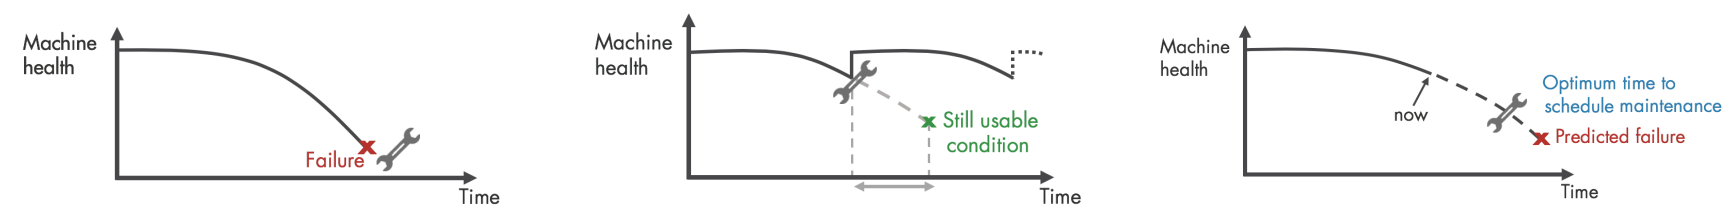
\includegraphics[width=1.1\textwidth]{maintenance.png}
    \caption{Reactive, preventive and predictive types of maintenance}
    \label{fig:maintenance}
\end{figure}


\paragraph{Fault Types} A fault is not an acceptable deviation of at least one
characteristic or parameter of the system from the standard condition.
There are different faults by their sources. 
\begin{itemize}
    \item Plant faults appear in system
        behavior and cause manufacturing performance.
    \item Component fault Actuator
    \item fault Sensor faults occurred in the sensor during measurements.
    \item Combination of faults
\end{itemize}
In many cases, faults lead to a system failure and
the system is no longer able to perform required functions.

Faults can be classified by the location where they appear, by a fault
form, or based on the form in which the fault is added to the system.


% -----------------------------------------------------------------------------
% 
% -----------------------------------------------------------------------------

\section{Fault Detection and Analysis (FDA)}

Fault Detection and Analysis, FDA (Fault Detection and Isolation, FDI) is a
subfield of control engineering focused on detecting the fault and
identifying where this fault is located. 
The main goals of FDI are
\begin{itemize}
    \item Fault detection, detect anomalies in real-time
    \item Fault isolation, find the root cause
    \item Fault identification, estimation of the magnitude, type, or nature of
        the fault 
\end{itemize}

Several methods are partly overlapped but divided into two main
categories. 

\paragraph{Signal-Based methods} Signal-Based methods (SB), explore measured
data and extract useful information in the form of features
\ref{fig:signal_based}. The following methods belong to the SB approach: 

\begin{itemize}
    \item Limit and trend checking
    \item Spectral analysis
    \item Data analysis (PCA)
    \item Pattern recognition
\end{itemize}

\begin{figure}[h!]
    \centering
    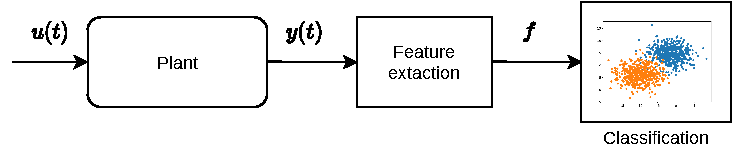
\includegraphics[width=0.7\textwidth]{signal_based.pdf}
    \caption{Signal-Based Method}
    \label{fig:signal_based}
\end{figure}


\paragraph{Model-Based methods} Model-Based methods exploit models identified
from real-life systems \ref{fig:model_based}. The model-based approach is
suitable when it is difficult to gain useful information using only
measured signals. If the system structure is known, it is possible to
extract features such as state variables or some system parameters. Typical
model-based techniques include

\begin{itemize}
    \item Residual estimation (compare measurements with "healthy" model)
    \item Polynomial coefficients
    \item State variables estimated using state observers
    \item Parameter estimation
\end{itemize}

\begin{figure}[h!]
    \centering
    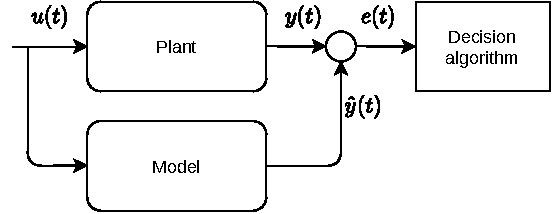
\includegraphics[width=0.5\textwidth]{model_based.pdf}
    \caption{Model-Based Method}
    \label{fig:model_based}
\end{figure}


Automated fault detection depends on input from sensors and postprocessing
algorithms. In many manufacturing applications, sensor failures are the
most common equipment failure.


The result of FDI is the detection and identification of faults that occur
during the operation of the device. Subsequently, predicted faults are
processed using fault tolerance and predictive maintenance algorithms.

\textbf{Fault Tolerance}: Provide the system with the hardware architecture
and software mechanisms that will allow, if possible, to achieve a given
objective in normal operation and given fault situations.

\subsection{Condition Monitoring}
Answer to question:"How does system operate now?"
CM gives Diagnostic methods that provides alarm or warning, but not
prognostic forecast about the future behavior (Not RUL).

But collected Condition Monitoring information can give information about
system degradation.


There is a optimization between technical and financial possibilities in a
specific situation.

FMECA (Failure Mode, Effect and Criticality Analysis) \\
FTA (Fault Tree Analysis) \\
RCA (Root Cause Analysis) \\


% -----------------------------------------------------------------------------
% 
% -----------------------------------------------------------------------------


\section{Predictive maintenance (PdM)}
\textbf{Predictive maintenance (PdM)} is cost-effective maintenance strategy that
predicts time to failure and warns of an anticipated location where this
could occur.

\subsection{Goals}
The are two main goals of Predictive maintenance, RUL (remaining useful
life) estimation and identification where the future failure can appear, or what is
the reason of decreasing RUL. 
As a result of PdM is RUL representing of number cycles, days, or some time
period before fault occurred. And probability where this fault can appear.

Predict where, when and what is the reason of failure (identify primary
factors).


\textbf{Predictive maintenance development sequence}:
\begin{enumerate}
    \item{Collect data (using sensors, math model)}
    \item{Process data (clean up data)}
    \item{Identify Condition Indicators CI}
        \begin{itemize}
            \item{Signal-based CI}
            \item{Model-based CI}
        \end{itemize}
    \item{Fit model (ML techniques)}
    \item{Deploy monitoring and integrate}
    \item{Dashboard (UI)}
\end{enumerate}


\subsection{Methods}
There are couples of signal processing and analyzing methods that used in
both PdM and FDI. For example:

\paragraph{Signal-Based} approach is suitable in situation when we have
measurements from system in different operating conditions. 
But there is a problem that Signal-Based approach enable to classify and
learn patterns observed in training dataset. 


\paragraph{Model-Based} approach is to use physical failure models. This
models do not require a large dataset of failure data. And they can work in
situations never observed before. 


%\begin{itemize}
%    \item Spectral Analysis
%    \item Wavelet Analysis
%    \item Wavelet transform
%    \item FFT
%    \item Short Term Fourier Transform
%    \item Gabor Expansion
%    \item Wigner-Ville distribution
%    \item Correlation
%    \item High resolution spectral analysis
%    \item Waveform Analysis
%    \item Time-Frequency Analysis
%    \item PCA
%    \item Machine Learning techniques:
%        \begin{itemize}
%            \item kNN
%            \item ANN
%        \end{itemize}
%\end{itemize}

\subsection{Condition Indicators}
Features in PdM field are called Condition Indicators or CI.
Condition Indicators are features extracted from the signals, representing some
system behavior and hides some information about system processing.

Condition indicators represented by three main domain. There are Time
domain, Frequency domain, Time-Frequency domain Condition Indicators.

\begin{itemize}
    \item Time-domain
    \item Frequency-domain
    \item Time-frequency
\end{itemize}

\subsection{Fault Classification}

\subsection{Remaining useful life}
RUL goal is remaining time before machine requires maintenance. Not only
predict but provide a confidence bound.

\paragraph{RUL Models}:
% https://www.mathworks.com/company/newsletters/articles/three-ways-to-estimate-remaining-useful-life-for-predictive-maintenance.html

Inputs are condition indicators and models depends on data: 1. Lifetime,
Run-to-failure, known threshold for CI.

\begin{itemize}
    \item Similarity model 
    \item Survival model
    \item Degradation model
\end{itemize}


\section{Digital twin}
% https://explore.mathworks.com/digital-twins-for-predictive-maintenance

Digital twin is digital representation of the real life system. Can be
represented as a component, a system of components, or as a system of
system.  

\paragraph{Updating digital twin with incoming data} 

Digital twin can be updated with incoming data from sensors. Fitting model
to new data, digital twin represents the current condition state of the
real world object.

%\todo[inline]{Rewrite}
Digital twin can hold historical data about behavior of a system
and can be used for simulation system operation in different conditions,
for designing control and simulate future behavior. (RUL, "What-if")

Digital Twins are helpful in the field of Anomaly Detection and Predictive
Maintenance.

Mathematical model of the real world system can be created using different
approaches. Modeling based on Physical modeling (Simscape) data-driven
modeling where system is represented as a "Black box" or some combination
of this approaches.
Model with estimated parameters uses for simulation system behavior in
different working conditions and with different faults during working
process.

\subsection{Using Digital Twin in PdM}

Measured data, Generated data from mathematical model, or Synthetic data
(Combination of measured and generated) can be used for assessment of
Condition Indicators. 

%\subsection{Detect and Diagnose Faults}
%Using condition indicators on Test data we can analyze actual system state.
%Designing algorithm is iterative process when you try different
%combinations of condition indicators and different models to evaluate best
%results.

\section{Comparison PdM and FDA approaches}

Figure 1 presents a relative arrangement of Predictive Maintenance (PdM) and
Fault Detection and Identification (FDI) algorithms. 

\begin{figure}[h!]
    \centering
    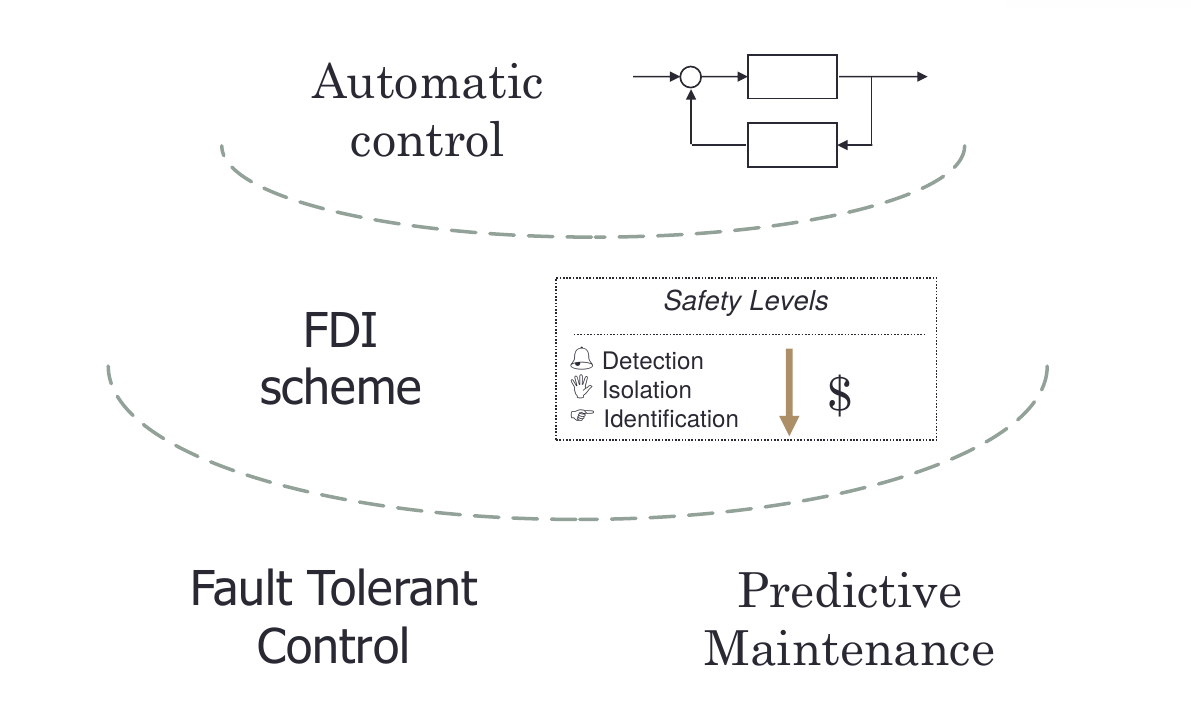
\includegraphics[scale=0.3]{FDI_PM.png}
    \caption{Relative arrangement of PdM and FDI algorithm}
    \label{fig:fdi_pm}
\end{figure}

\begin{itemize}
    \item Compare similarities and differences in FDA and PdM
\end{itemize}

\section{Application field}
\begin{itemize}
    \item Answer to question where FDA and PdM can be suitable.
\end{itemize}
